\documentclass[11pt]{article}
\usepackage{amsmath,amssymb}
\usepackage[margin=1in]{geometry}
\usepackage{tikz}
\usetikzlibrary{positioning,arrows.meta}
\title{DQN 3-Layers Vectorial}
\author{}
\date{}
\begin{document}
\maketitle

\section{Network}
Fully linear Q-network (no activation). Architecture:
\begin{center}
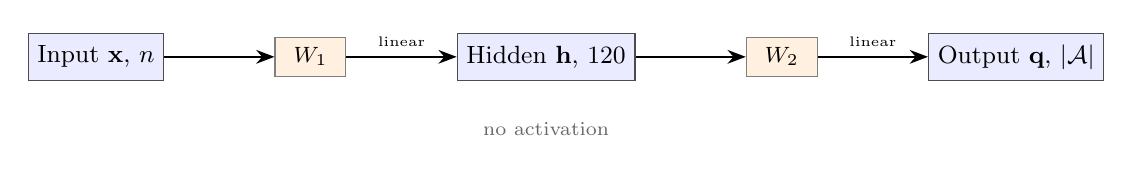
\begin{tikzpicture}[
  node distance=1.4cm,
  layer/.style={rectangle, draw=black!70, fill=blue!8, minimum width=1.4cm, minimum height=0.6cm, font=\small},
  weight/.style={rectangle, draw=black!50, fill=orange!12, minimum width=0.9cm, minimum height=0.5cm, font=\footnotesize},
  arrow/.style={-Stealth, thick}
  ]
  \node[layer] (in) {Input $\mathbf{x}$, $n$};
  \node[weight, right=of in] (w1) {$W_1$};
  \node[layer, right=of w1] (hid) {Hidden $\mathbf{h}$, 120};
  \node[weight, right=of hid] (w2) {$W_2$};
  \node[layer, right=of w2] (out) {Output $\mathbf{q}$, $|\mathcal{A}|$};
  \draw[arrow] (in) -- (w1);
  \draw[arrow] (w1) -- (hid) node[midway, above, font=\tiny] {linear};
  \draw[arrow] (hid) -- (w2);
  \draw[arrow] (w2) -- (out) node[midway, above, font=\tiny] {linear};
  \node[below=0.4cm of hid, font=\scriptsize, text=black!60] {no activation};
\end{tikzpicture}
\end{center}

\noindent Equations:
\begin{equation}
\mathbf{h} = W_1 \mathbf{x} + \mathbf{b}_1, \qquad
\mathbf{q} = W_2 \mathbf{h} + \mathbf{b}_2
\end{equation}
with $\mathbf{x} \in \mathbb{R}^n$, $\mathbf{h} \in \mathbb{R}^{120}$, $\mathbf{q} \in \mathbb{R}^{|\mathcal{A}|}$. So
\begin{equation}
Q(s,a) = \mathbf{q}_a = (W_2 W_1)_{a,:} \mathbf{x} + \text{bias}_a.
\end{equation}

\section{Feature contribution}
Effective weight from input to Q per action:
\begin{equation}
W_{\text{eff}} = W_2 W_1 \quad \in \mathbb{R}^{|\mathcal{A}| \times n}.
\end{equation}
Contribution of feature $i$ to action $a$ (additive term in $Q(s,a)$):
\begin{equation}
c_{a,i}(s) = (W_{\text{eff}})_{a,i} \, x_i.
\end{equation}
For chosen action $a_b$ in a batch: $\mathbf{c}_b = (W_{\text{eff}}[a_b,:]) \odot \mathbf{x}_b$.

\section{Vectorial reward}
Per-feature reward (reward backpropagated to features):
\begin{equation}
r_{\text{vec},i} = \frac{r}{n} \quad \forall i.
\end{equation}
So $\mathbf{r}_{\text{vec}} \in \mathbb{R}^n$ has each entry $r/n$.

\section{Loss}
TD target (no gradient):
\begin{equation}
y = r + \gamma \, \max_{a'} Q_{\text{target}}(s',a') \cdot (1 - \text{done}).
\end{equation}
TD loss:
\begin{equation}
L_{\text{td}} = \frac{1}{B} \sum_{b=1}^{B} \bigl( y_b - Q(s_b, a_b) \bigr)^2.
\end{equation}
Per-feature loss (contribution of feature $i$ to chosen action vs $r/n$):
\begin{equation}
L_i = \frac{1}{B} \sum_{b=1}^{B} \bigl( c_{b,i} - \tfrac{r_b}{n} \bigr)^2.
\end{equation}
Vectorial loss and total loss:
\begin{equation}
L_{\text{vec}} = \frac{1}{n} \sum_{i=1}^{n} L_i, \qquad
L = L_{\text{td}} + \lambda \, L_{\text{vec}}.
\end{equation}
$\lambda$ is \texttt{vectorial\_loss\_coef} (default $0.1$).

\subsection{How the loss connects to the architecture}
\begin{center}
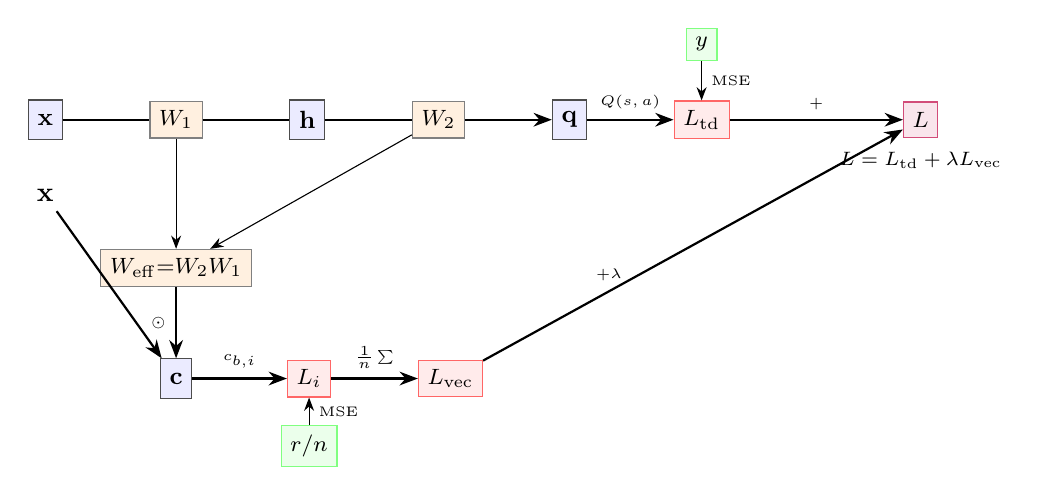
\begin{tikzpicture}[
  node distance=0.9cm and 1.1cm,
  layer/.style={rectangle, draw=black!70, fill=blue!8, minimum height=0.5cm, font=\small},
  weight/.style={rectangle, draw=black!50, fill=orange!12, minimum height=0.45cm, font=\footnotesize},
  lossbox/.style={rectangle, draw=red!60, fill=red!8, minimum height=0.45cm, font=\footnotesize},
  target/.style={rectangle, draw=green!50, fill=green!8, minimum height=0.4cm, font=\footnotesize},
  arrow/.style={-Stealth, thick},
  smallarrow/.style={-Stealth, font=\tiny}
  ]
  % Row 1: forward pass and L_td
  \node[layer] (x) {$\mathbf{x}$};
  \node[weight, right=of x] (w1) {$W_1$};
  \node[layer, right=of w1] (h) {$\mathbf{h}$};
  \node[weight, right=of h] (w2) {$W_2$};
  \node[layer, right=of w2] (q) {$\mathbf{q}$};
  \node[lossbox, right=of q] (ltd) {$L_{\mathrm{td}}$};
  \node[target, above=0.5cm of ltd] (y) {$y$};
  \draw[arrow] (x) -- (w1) -- (h) -- (w2) -- (q);
  \draw[arrow] (q) -- (ltd) node[midway, above, font=\tiny] {$Q(s,a)$};
  \draw[smallarrow] (y) -- (ltd) node[midway, right, font=\tiny] {MSE};

  % Row 2: W_eff and contributions -> L_i, L_vec
  \node[weight, below=1.4cm of w1] (weff) {$W_{\mathrm{eff}}{=}W_2 W_1$};
  \node[below=0.5cm of x] (x2) {$\mathbf{x}$};
  \node[layer, below=of weff] (c) {$\mathbf{c}$};
  \node[lossbox, right=1.2cm of c] (li) {$L_i$};
  \node[lossbox, right=of li] (lvec) {$L_{\mathrm{vec}}$};
  \node[target, below=0.35cm of li] (rvec) {$r/n$};
  \draw[smallarrow] (w1) -- (weff);
  \draw[smallarrow] (w2) -- (weff);
  \draw[arrow] (x2) -- (c);
  \draw[arrow] (weff) -- (c) node[midway, left, font=\tiny] {$\odot$};
  \draw[arrow] (c) -- (li) node[midway, above, font=\tiny] {$c_{b,i}$};
  \draw[smallarrow] (rvec) -- (li) node[midway, right, font=\tiny] {MSE};
  \draw[arrow] (li) -- (lvec) node[midway, above, font=\tiny] {$\frac{1}{n}\sum$};

  % Total loss
  \node[lossbox, draw=purple!70, fill=purple!10, right=2.2cm of ltd] (L) {$L$};
  \draw[arrow] (ltd) -- (L) node[midway, above, font=\tiny] {$+$};
  \draw[arrow] (lvec) -- (L) node[pos=0.3, above, font=\tiny] {${+}\lambda$};
  \node[below=0.05cm of L, font=\scriptsize] {$L = L_{\mathrm{td}} + \lambda L_{\mathrm{vec}}$};
\end{tikzpicture}
\end{center}
\noindent\textbf{Top row:} Forward pass $\mathbf{x} \to W_1 \to \mathbf{h} \to W_2 \to \mathbf{q}$; $Q(s,a)$ is the chosen action's value; $L_{\mathrm{td}}$ is MSE between $Q(s,a)$ and TD target $y$. \textbf{Bottom row:} $W_{\mathrm{eff}} = W_2 W_1$ gives per-feature contribution $\mathbf{c} = W_{\mathrm{eff}}[a,:] \odot \mathbf{x}$; each $L_i$ is MSE between $c_{b,i}$ and $r/n$; $L_{\mathrm{vec}} = \frac{1}{n}\sum_i L_i$. \textbf{Total:} $L = L_{\mathrm{td}} + \lambda L_{\mathrm{vec}}$ is backpropagated through the network to update $W_1$, $W_2$.
\end{document}
